\mychapter{Introdução e Delimitação do Problema}{chp:Fundamentação Teórica}
\lhead{Introdução e Delimitação}

% Breve resumo do capítulo.
\lettrine{E}{ste} capítulo tem como objetivo apresentar uma fundamentação teórica necessária para embasar os conceitos aplicados no trabalho.
Delimitaremos aqui o problema a ser tratado nesta tese.

Em relação a fundamentação teórica, utilizou-se como principal fonte de pesquisa a área de indexação de periódicos científicos ISI \emph{Web of Knowledge}, onde foram obtidas a grande maioria das referências, usando como parâmetros o fator de impacto dos periódicos pesquisados, a quantidade de citações de cada publicação, o grau de relevância para o tema pesquisado e o nível de produtividade (fator-H) dos autores envolvidos. 
O apoio em livros, \textit{surveys}, \textit{lecture notes} e ferramentas complementares de busca, como o \emph{Google Acadêmico} foram utilizadas para complementar esta pesquisa.

\section{Números Aleatórios} %Simulação física, Von Neumann, Congruenciais Lineares, etc

A noção de aleatoriedade é fundamental em diversas áreas, entretanto uma definição precisa, até mesmo do ponto de vista matemático rigoroso, é bastante difícil. 
Algumas questões emergem naturalmente como, o que vem a ser aleatoriedade? 
Existem eventos aleatórios na natureza? 
Faz algum sentido buscar leis da aleatoriedade? 
É possível simular a aleatoriedade? 
Estas são questões muito difíceis, envolvendo, inclusive, os primórdios da investigação filosófica como discute \citep{Volchan:02}.
Essa dificuldade é bem ilustrada de forma humorística na Figura~\ref{fig:Dilbert}.

\begin{figure}[hbt]
\centering
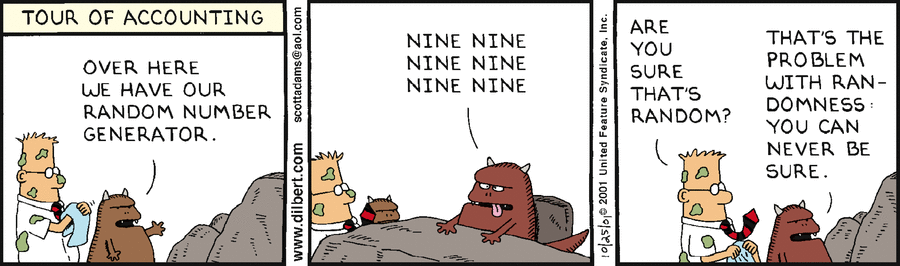
\includegraphics[width=.7\linewidth]{dilbert}
\caption{Visão de Dilbert de um gerador de números aleatórios}\label{fig:Dilbert}
\end{figure}

Números aleatórios perfazem uma das partes mais importantes em aplicações computacionais nos vários campos do conhecimento, como aborda \citep{Knuth:98}:
\begin{itemize}
     \item \textit{Simulação} - Quando um computador é usado para simular fenômenos naturais, números aleatórios são necessários para fazer as coisas de forma realística. Simulação abrange diversas áreas, desde o estudo de física nuclear (onde particulas são submetidas a colisões aleatórias) até pesquisa operacional (como, por exemplo, a taxa de pessoas que entram num aeroporto em intervalos aleatórios).
     \item \textit{Amostragem} - É praticamente impossível examinar todos os possíveis casos, porém uma amostra aleatória provê um palpite sobre como é o comportamento típico do fenômeno em questão.
     \item \textit{Análise Numérica} - Técnicas elaboradas para a solução de complexos problemas numéricos foram desenvolvidas utilizando-se números aleatórios.
     \item \textit{Programação de Computadores} - Valores aleatórios são uma ótima fonte de dados para testar a eficácia de algoritimos computacionais.
     \item \textit{Tomada de Decisão} - Existem relatos de que diversos executivos tomam suas decisões lançando moedas ou atirando dardos. Também há rumores de que professores universitários lançam suas notas de forma similar. Em alguns momentos é importante tomar decisões de forma não influenciada por qualquer agente externo.
     \item \textit{Criptografia} - Uma fonte de bits não viesada é essencial para diversos tipos de comunicações seguras, quando os dados precisam ser mantidos em sigilo.
     \item \textit{Estética} - Um pouco de aleatoriedade faz com que gráficos e músicas geradas por computador aparentem ser menos artificiais.
     \item \textit{Diversão} - Rolar dados, embaralhar cartas, girar rodas de roletas, etc., são passatempos facinantes para muitos. Estes usos tradicionais de números aleatórios sugeriram o nome ``Método de Monte Carlo''.
    \end{itemize}

Existem dois tipos básicos de geradores utilizados para produzir sequências aleatórias: GNAs -- Geradores de Números Aleatórios, do inglês (\textit{RNGs} -- \textit{Random Number Generators}) e GNPA -- Geradores de Números Pseudoaleatórios, do inglês (\textit{PRNGs} -- Pseudorandom Number Generators).

\subsection{Geradores de Números Aleatórios -- GNA}
  
Geradores de Números Aleatórios utilizam uma fonte não determinística juntamente com algumas funções de processamento para produzir aleatoriedade. 
As saídas deste tipo de gerador podem ser usadas diretamente como números aleatórios, desde que satisfaçam critérios de aleatoriedade, ou ainda podem servir como parâmetro de entrada para geradores de números pseudoaleatórios, vistos com mais detalhes na sequência. 

A maior parte dos geradores utiliza-se de fenômenos físicos naturais como, decaimento radioativo, ruidos termais em semiconcutores, amostras de som num local ruidoso, ruído no espectro eletromagnético, dentre outros que, por óbvia dedução, carecem de algum hardware específico para serem capturados. 

Na literatura é possível encontrar trabalhos relatando detalhadamente a criação de geradores de números aleatórios utilizando fontes de aleatoriedade apropriadas.
\citet{Fairfield:85} descrevem a geração de um fluxo de bits aleatórios baseado na instabilidade da frequência de um oscilador.
Evidentemente a construção de um gerador como o descrito anteriormente demanda o emprego de técnicas apuradas e um grande conhecimento teórico, além de necessitar, em sua grande maioria, de hardware especializado, o que gera uma barreira para os usuários que demandam tais dados aleatórios.
Desta sorte, frequentemente os usuários precisam se valer de técnicas alternativas para obter aleatoriedade.

\subsection{Geradores de Números Pseudoaleatórios -- GNPA}

Dadas as dificuldades descritas anteriormente, atualmente a maneira mais conveniente e confiável de se gerar números aleatórios para diversas aplicações é através de algoritmos com um sólido embasamento matemático. 
Tais algoritmos produzem sequências de números sabidamente não aleatórios ao todo, mas que aparentam comportar-se como números aleatórios independentes, isto é, tomada uma sequência de variáveis aleatórias independentes e identicamente distribuídas sobre o Intervalo $(0,1)$. 
Tal sequência pode ser chamada de ``Pseudoaleatória'' e o programa utilizado em sua produção de ``Gerador de Números Pseudoaleatórios'' como define \citet{LEcuyer:98}.

\section{Principais Testes Clássicos} %Revisão Cronológica/Conceitual

Existem duas abordagens para testar-se a capacidade de geradores aleatórios ou pseudoaleatórios produzirem sequências ditas aleatórias.
Segundo \citet{LEcuyer:92} são elencados em teóricos e empíricos.

Os testes teóricos são bastante específicos para cada tipo de GNPA, pois analisam o as propriedades das sequências a partir da definição do gerador.
Já os testes empíricos valem-se de técnicas estatísticas objetivando avaliar o quão boas são as sequências produzidas por um determinado gerador.
Estes últimos podem ser aplicados tanto a GNAs quanto a GNPAs.

Neste trabalho propomos um teste empírico não paramétrico baseado em ferramentas da teoria da informação.
A seguir daremos uma breve introdução aos testes disponíveis na literatura e ao estado da arte.
  
% \subsection{Diehard}
 
 \subsection{NIST}
 
Fundado em 1991, o NIST (\textit{National Institute of Standards and Technology}) é uma agência não regulatória do Departamento de Comércio dos Estados Unidos da América que tem por missão promover a inovação e a competitividade nos EUA através da ciência de medidas, padrões e tecnologia de forma a alavancar a segurança econômica e melhorar a qualidade de vida do povo americano.

A sua Divisão de Segurança de Computadores (CSD) e o Centro de Pesquisa em Segurança Computacional (CSRC) facilitam a ampla disseminação de práticas e ferramentas de segurança da informação, provendo recursos para a definição de padrões além de identificar recursos de segurança na Web para suportar usuários na industria, governo e academia. 

CSRC é o portal de acesso primário para se ter acesso às publicações de segurança de computadores, padrões e instruções, além de outras informações relacionadas a segurança.

Desde 1997, o Grupo de Trabalho Técnico em Geração de Números Aleatórios (RNG-TWG) tem trabalhado no desenvolvimento de uma bateria de testes estatísticos apropriados para a avaliação de geradores de números aleatórios e pseudoaleatórios utilizados em aplicações criptográficas. 

Os principais objetivos do grupo são:
  \begin{itemize}
   \item Desenvolvimento de uma bateria de testes estatísticos para detectar não aleatoriedade em sequencias binárias construidas através de geradores de números aleatórios e pseudoaleatórios utilizados em aplicações criptográficas;
   \item Produzir documentação e uma implementação em software destes testes;
   \item Prover auxílio no uso e aplicação destes testes.
  \end{itemize}

\subsection{Diehard e Dieharder}

George Marsaglia desenvolveu a bateria de testes Diehard em 1995, e os disponibilizou em CD-ROM.
Robert Brown identificou limitações nessa bateria de testes, os implementou novamente na linguagem de programação C, acrescentou testes da bateria NIST e disponibilizou um conjunto ampliado de testes denominado Dieharder.
A página Web \url{http://webhome.phy.duke.edu/~rgb/General/dieharder.php} é o portal de acesso a esses testes bem como a resultados de aplicá-los a diversas fontes de dados.

\subsection{ENT}

ENT \citet{ENTTestSuite} realiza uma variedade de testes no fluxo de bytes de um arquivo (ou na entrada padrão se nenhum arquivo for especificado) e produz uma saída como esta:

\begin{verbatim}
Entropy = 7.980627 bits per character.

Optimum compression would reduce the size
of this 51768 character file by 0 percent.

Chi square distribution for 51768 samples is 1542.26, and randomly
would exceed this value less than 0.01 percent of the times.

Arithmetic mean value of data bytes is 125.93 (127.5 = random).
Monte Carlo value for Pi is 3.169834647 (error 0.90 percent).
Serial correlation coefficient is 0.004249 (totally uncorrelated = 0.0).
\end{verbatim}

ENT é distribuido em forma de binário para a plataforma Win32 e pode ter descarregado o seu código fonte para construção sob ambiente \textit{Unix-Like}
  
\subsection{TestU01}	

Considerado como o estado da arte dos testes para geradores de números aleatórios \citet{LEcuyer:07}, o $TestU01$ se apresenta como uma biblioteca de software escrita em $ANSI$ $C$ que oferece uma coleção de utilitários para testagem, ele provê implemetações generalistas dos testes estatísticos clássicos para geradores de números aleatórios, bem como de vários outros propostos na literatura, além de propor alguns originais. Pode ser aplicado a números aleatórios produzidos por qualquer tipo de dispositivo ou armazenados em arquivos.

O principal problema com o uso dos testes NIST, Dieharder, Test$U01$ e outros similares é que estão direcionados a usuários especializados.
Uma parcela significativa de pesquisadores prefere ferramentas visuais, como a descrita a seguir.

\subsection{Visualização}

O intuito desses testes é a verificação de que os dados produzidos por um gerador, seja ele algoritmico ou físico, não se afastam significativamente da hipótese de serem eventos de variáveis independentes e identicamente distribuídas segundo uma lei Uniforme no intervalo $(0,1]$.

Verificar que os dados seguem uma lei Uniforme é relativamente simples, e há para eles uma bateria de testes que observam diversas propriedades.

A componente mais difícil é a de verificar a independência, por se tratar de independência coletiva e não apenas aos pares.

A falta de independência de uma sequência de $N$ pontos pode se manifestar de várias maneiras.
Uma delas é quando os pontos jazem em subespaços de dimensão menor a $N$, ao invés de preencher o espaço por completo.

As figuras~\ref{fig:3DMT} e~\ref{fig:3DRandu} mostram sequências de três pontos não sobrepostos desenhadas no cubo unitário.
A primeira perspectiva (figs.~\ref{MTa} e~\ref{Ra}) mostram uma perspectiva dos pontos que não levanta nenhuma suspeita.
Já as figuras~\ref{MTb} e~\ref{Rb} mostram que as sequências produzidas pelo gerador RANDU não preenchem o espaço, mas ficam confinadas a alguns planos, enquanto que as produzidas por Mersenne-Twister não apresentam essa deficiência.

\begin{figure}[hbt]
\centering
\subfigure[Primeira perspectiva\label{MTa}]{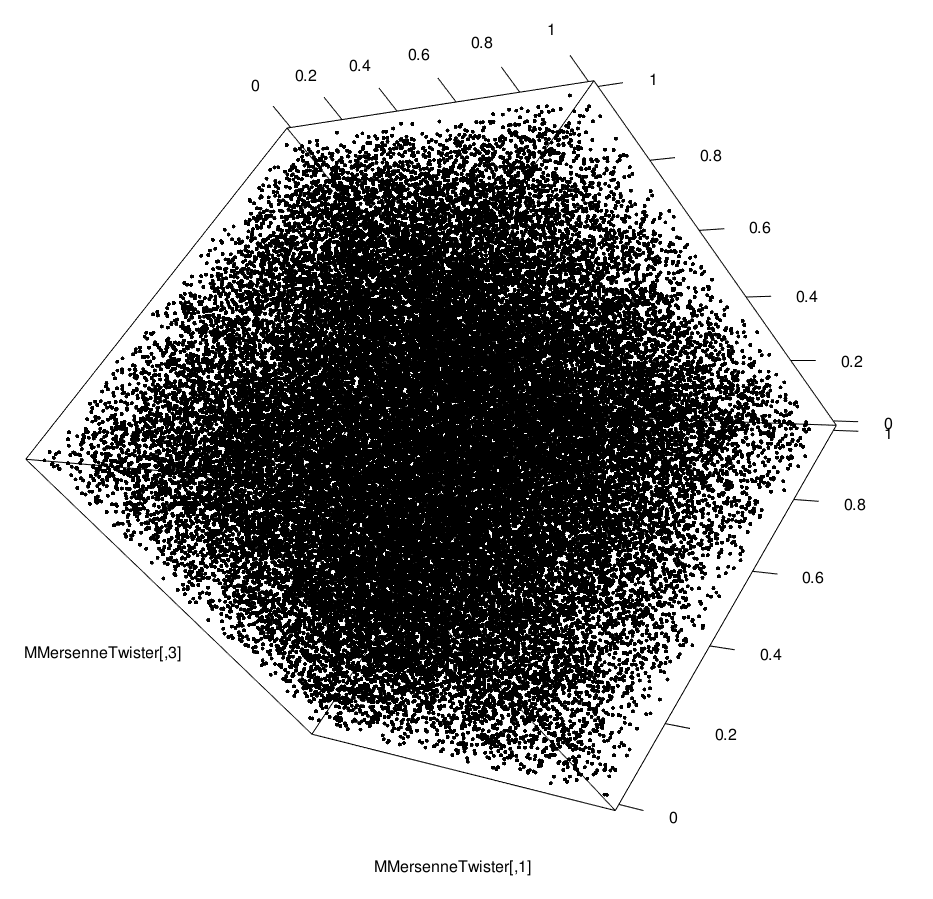
\includegraphics[width=.48\linewidth]{MT3D}}
\subfigure[Segunda perspectiva\label{MTb}]{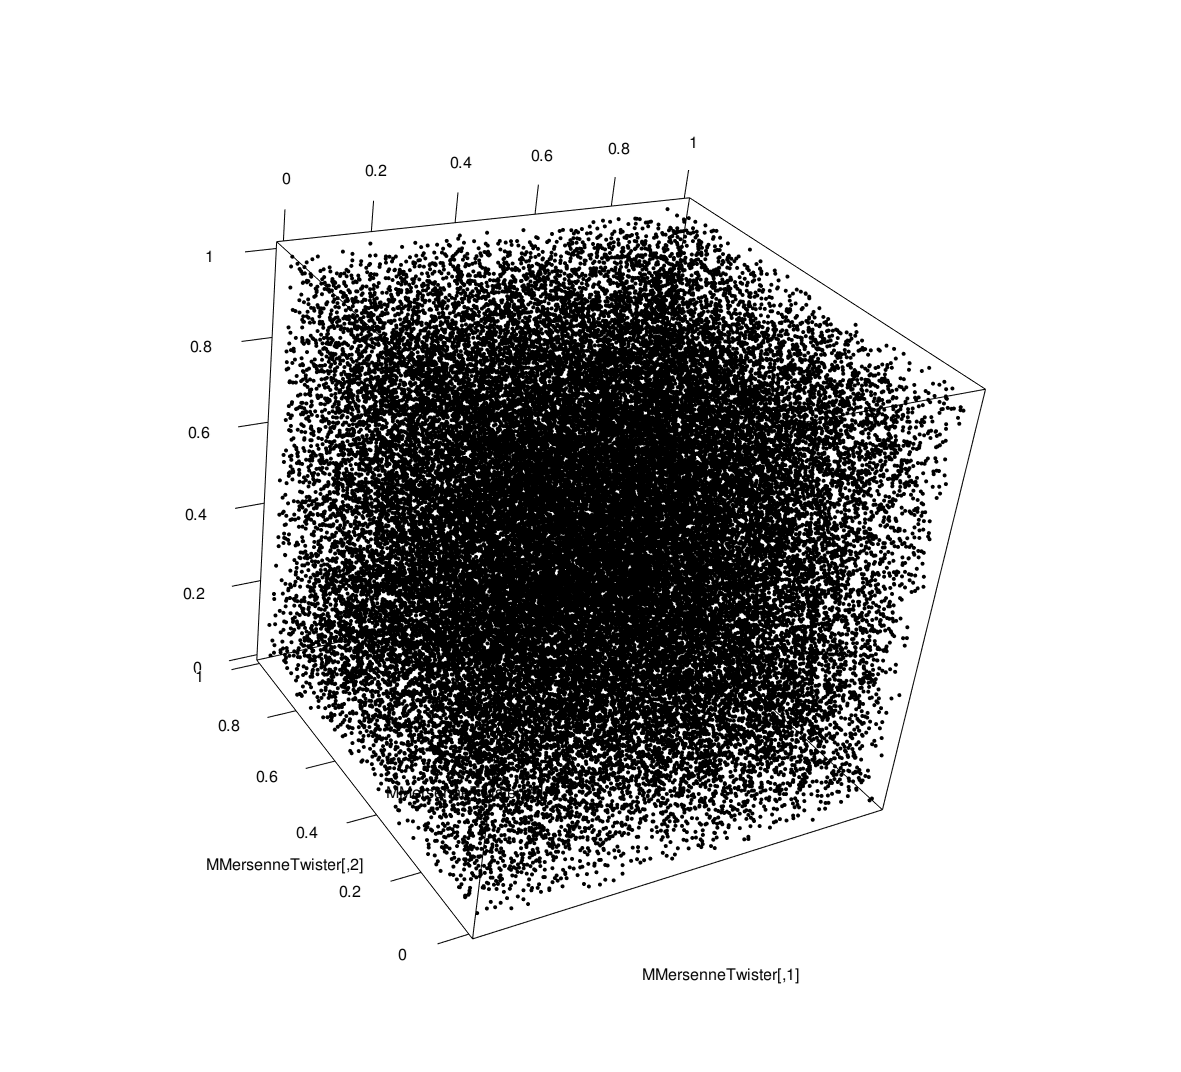
\includegraphics[width=.48\linewidth]{MT3Dsubspace}}
\caption{Visualização 3D de sequências disjuntas produzidas pelo gerador Mersenne-Twister}\label{fig:3DMT}
\end{figure}

\begin{figure}[hbt]
\centering
\subfigure[Primeira perspectiva\label{Ra}]{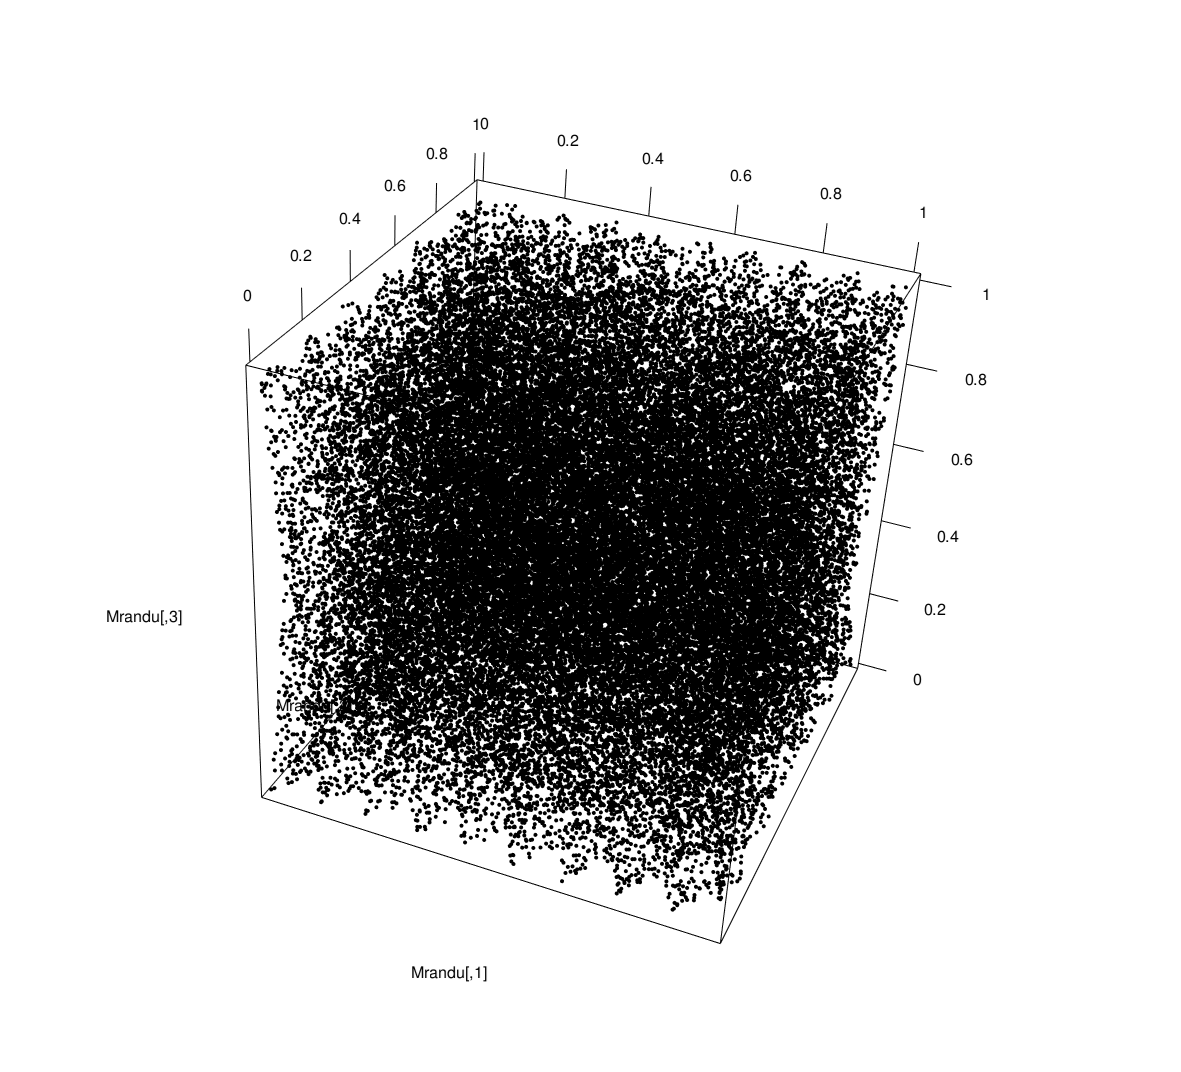
\includegraphics[width=.48\linewidth]{Randu3D}}
\subfigure[Segunda perspectiva\label{Rb}]{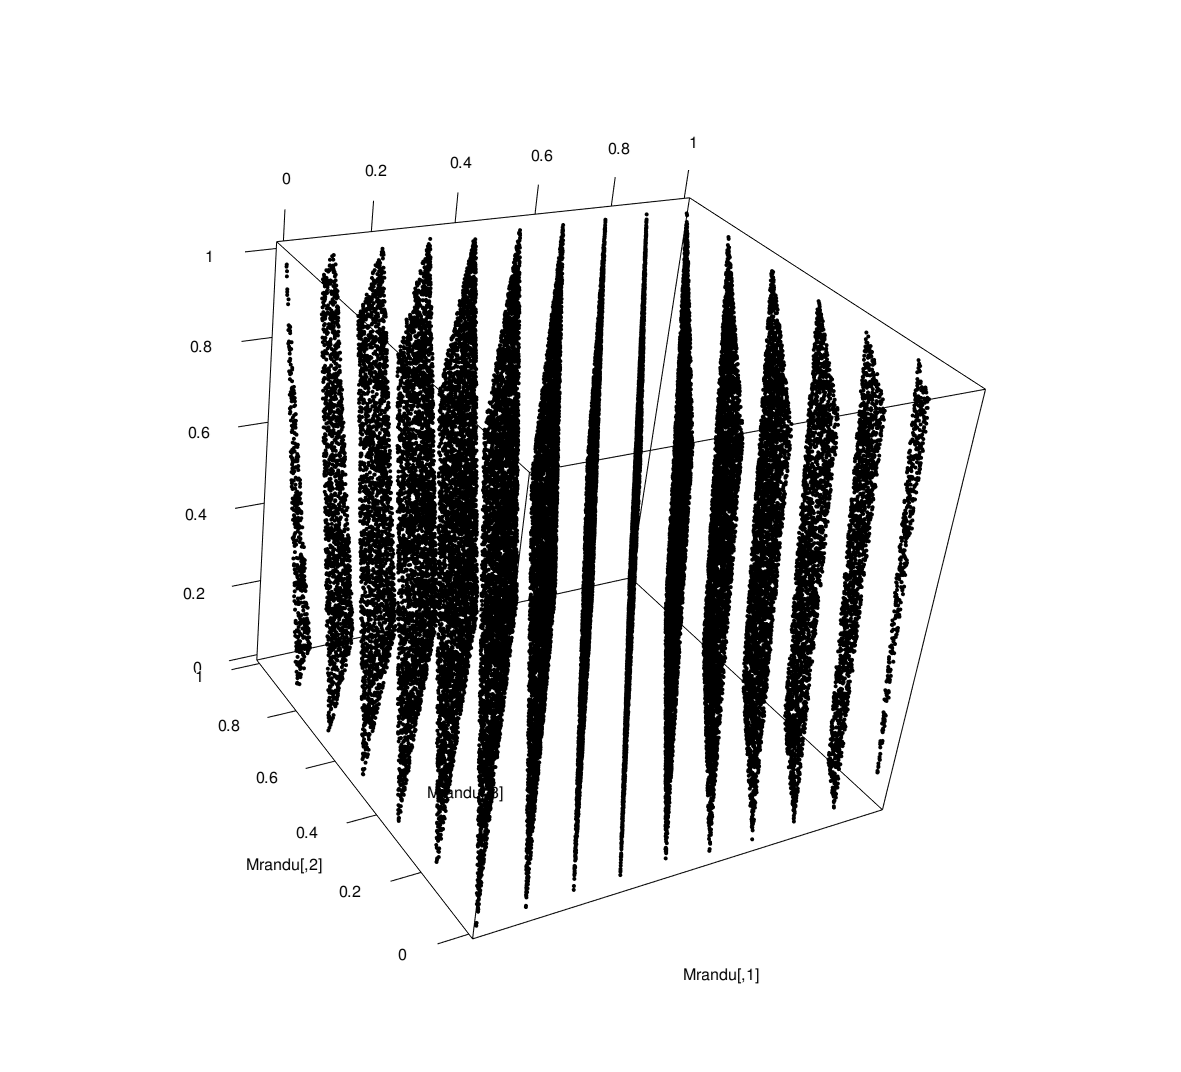
\includegraphics[width=.48\linewidth]{Randu3Dsubspace}}
\caption{Visualização 3D de sequências disjuntas produzidas pelo gerador RANDU}\label{fig:3DRandu}
\end{figure}

Embora o exemplo mostre claramente que o gerador RANDU apresenta problemas, nem sempre é fácil identificar esse tipo de estrutura.
Isso se deve a que ela pode ocorrer em espaços de dimensão maior, ou seguindo estruturas mais complexas.

\subsection{Descritores baseados em Teoria da Informação}

O trabalho pioneiro de \citet{PermutationEntropyBandtPompe} representa uma mudança de paradigma na análise de séries temporais, e será o nosso marco referencial teórico.

Eles propõem uma técnica não-paramétrica de análise de sequências que consiste em transformar palavras de $D$ dados não necessariamente subsequentes em símbolos ordinais.
Esses símbolos codificam a ordem que as $D$ observações têm na sequência e, portanto, são bem menos sucetíveis a contaminação dos que os próprios valores.
Forma-se então um histograma de proporções dos símbolos observados, e calculam-se duas quantidades: a Entropia e a Divergência de Jensen-Shannon a uma distribuição de referência (usualmente a uniforme).
A série, finalmente, é representada pelo par de valores Entropia-Complexidade Estatística, sendo que esta última é o produto da Entropia e a Divergência de Jensen-Shannon.

O conjunto de valores possíveis dos pontos característicos de qualquer série não varre $\mathbbm R^2$, mas constitui-se em um subconjunto compacto do plano: o plano Entropia-Complexidade, visto na Figura \ref{fig:Plano_HC}.
\begin{figure}[hbt]
	\centering
	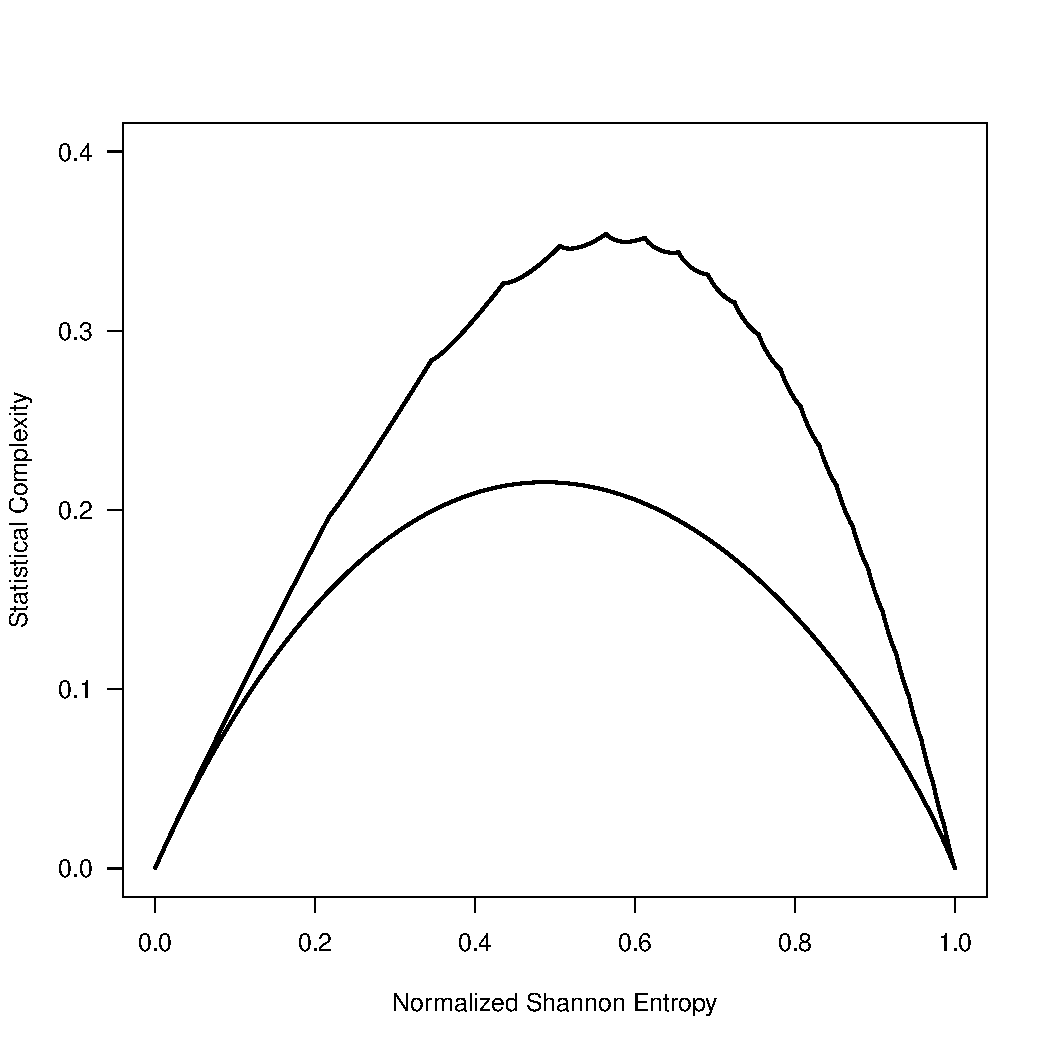
\includegraphics[width=.7\linewidth]{plano_HC}
	\caption{Plano Entropia-Complexidade.}\label{fig:Plano_HC}
\end{figure}
Uma grande quantidade de trabalhos mostra que a posição dos pontos característicos no plano Entropia-Complexidade é capaz de caracterizar diversos tipos de dinâmicas, sendo as duas extremas o ponto $(0,0)$, que corresponde a sequências determinísticas, e o ponto $(1,0)$, típico de ruído branco.

Alguns dos trabalhos emblemáticos que empregam essa abordagem são:
\begin{description}
\item[\citet{RandomNumberGeneratorsCausality}] mostram que o plano Entropia-Complexidade permite prever o resultado dos testes Diehard de qualidade de GNPA.
\item[\citet{GeneralizedStatisticalComplexityMeasuresGeometricalAnalyticalProperties}] analisam o mapa caótico logístico e discutem cotas no plano Entropia-Complexidade.
\item[\citet{EEGAnalysisWaveletInformationTools}] analisam dados de eletroencefalogramas de pacientes com epilepsia 	utilizando decomposição wavelet e o plano Entropia-Complexidade.
\item[\citet{De_Micco_2008}] avaliam melhorias da qualidade de sequências pseudoaleatórias.
\item[\citet{De_Micco_2009}] estudam as componentes caóticas de GNPAs.
\item[\citet{ComplexNetworksEvolution}] analisam a evolução de redes dinâmicas com descritores baseados em Teoria da Informação.
\item[\citet{DistinguishingChaoticStochasticDynamicsTimeSeriesMultiscaleSymbolicApproach}] analisam a relação entre dinâmicas caóticas e estocásticas com uma abordagem multiescala.
\item[\citet{StructuralChangesDataCommunicationWSN}] utilizam descritores de Teoria da Informação para descrever a dinâmica de redes de sensores sem fios.
\item[\citet{DistinguishingNoiseFromChaos}] caracterizam sequências com componentes caóticas e estocásticas no plano Entropia-Complexidade.
\item[\citet{CharacterizationVehicleBehaviorInformationTheory}] analisam o comportamento de veículos em larga escala em função da topologia de diversas cidades.
\item[\citet{DiagnosingDynamicsObservedSimulatedEcosystem}] analisam séries temporais de fenômenos ambientais.
\item[\citet{InformationTheoryPerspectiveNetworkRobustness}] verificam o efeito de ataques em redes complexas através de descritores no plano Entropia-Complexidade.
\item[\citet{ClassificationVerificationOnlineHandwrittenSignatures}] mostram a expressividade dos descritores de Teoria da Informação para o problema de classificação e verificação de assinaturas.
\item[\citet{CharacterizationElectricLoadInformationTheoryQuantifiers}] conseguem caracterizar o tipo de dispositivo elétrico observando o ponto no plano Entropia-Complexidade em que o histórico do seu consumo é mapeado.
\end{description}

Uma limitação de todos esses trabalhos é que os pontos no plano são atribuídos a padrões prototípicos, isto é, a modelos, de forma \textit{ad hoc}.
O autor desta dissertação só conhece um trabalho em que é feita uma análise da significância da posição de pontos característicos no plano Entropia-Complexidade: o artigo de \citet{NewPermutationEntropy}.

Nesse contexto, esta dissertação fornece regiões de confiança para uma boa diversidade de situações que permitem verificar a significância da hipótese de uma sequência aleatória ou pseudoaleatória é aderente à hipótese dela ser ruído branco.

\section{Delimitação do problema} %Delimitação do problema  

A motivação deste trabalho é o desenvolvimento de um teste baseado em Teoria da Informação para verificar a hipótese de que uma sequência é ruído branco, isto é, formada por observações de variáveis aleatórias independentes e identicamente distribuídas.
Para tanto, trabalharemos com atributos derivados da simbolização de Bandt \& Pompe.
Cada sequência sob análise será transformada em um ponto no plano Entropia-Complexidade, e será medida a sua distância ao ponto característico de sequências ideais.
Analisaremos, então, a distribuição empírica de uma variedade de situações de interesse para, finalmente, propor regiões de confiança da hipótese nula.
Por fim, analisaremos sequências com o ferramental aqui proposto.
